\documentclass{article}
\usepackage{graphicx} % Required for inserting images
\graphicspath{ {figures/} }
\usepackage{array}
\usepackage{float}
\usepackage{caption}
\usepackage{amsmath}
\usepackage{amsfonts}
\newcommand{\C}{{\mathbb C}}
\newcommand{\E}{{\mathbb E}}
\newcommand{\R}{{\mathbb R}}
\newcommand{\Prr}{{\mathbb P}}
\newcommand{\N}{{\mathbb N}}
\newcommand{\D}{{\mathbb D}}
\newcommand{\Z}{{\mathbb Z}}
\usepackage{hyperref}
\usepackage{pgfplotstable}
\pgfplotsset{compat=1.18}
\usepackage{booktabs}
\usepackage{array}
\usepackage{colortbl}
\usepackage{amsthm}
\newtheorem{theorem}{Theorem}[section]
\newtheorem{lemma}[theorem]{Lemma}
\newtheorem{remark}{Remark}
\newtheorem{note}{Note}[section]

% Redefine the format for figure captions
\captionsetup[figure]{
    labelfont={bf},   % Make the label bold (e.g., "Figure 1")
    labelsep=colon,   % Set the separator after the label (optional, default is a colon)
}


\title{Multiperiod Collection of Results}
\author{Prof. Serhiy Kozak \& James Zhang}
\date{\today}

\begin{document}

\maketitle

\tableofcontents

\newpage

\section{Setup}

All $R$ tensors are \emph{log} returns, not simple and not excess of the one-lag return \footnote{Clarify that returns are excess of the risk-free rate, they should be, I know it is for the Characteristics Anomalies dataset}. 
The out-of-sample period for all datasets is 
post January 2005. \footnote{We should standardize this to be 01-31-2005 to 2020-08-01, but in the preliminary, should not be a huge difference across 
the datasets.} In our primary specification, 

\begin{itemize}
    \item Rolling window size $W$ is fixed at $120$ months.
    \item Maximum horizon $S$ is fixed at $36$ months.
    \item Maximum lag (lagged characteristics) is $36$ months.
    \item For each dataset and setting, we experiment with $K = 1, 3, 5, 10, 15, 20, 25$, where 
    $K$ represents the rank of PARAFAC and PCA ie. the number of factors.
extracted from the tensor or matrix, respectively. 
    \item Default $\gamma = 0$, we do not yet experiment with RP-PCA in the MVE procedure.
\end{itemize}

For robustness purposes, we present multiperiod results for each of the following $3$ datasets:

\begin{enumerate}
\item Characteristics Anomalies dataset: 1972-06-01 (ie. $\min(t - L)$)  to 2020-08-01
.
- $43$ characteristic-sorted portfolios (SortedFactors)

\item SCS dataset: 1972-07-31 to 2021-12-31

- $44$ characteristic-based portfolios (UnivariateFactors). All industry and constant factors are now removed.

\item WRDS dataset: 1975-01-31 to 2020-12-31

- $107$ characteristic-based portfolios (UnivariateFactors). I believe this dataset still currently has imputed data points, so we should get a version of this with $0$ imputed data points.


\end{enumerate}

For the Characteristic Anomalies dataset, factors are decile-sorted long-short portfolios. For the SCS and WRDS datasets, 
each stock is weighted by its characteristic signal value
and signals are based on cross-sectional ranks, centered and normalized. 


\section{Models}

\subsection{Tensor Factor Model (Approximate)} \label{approx}

This is the primary model outlined in the paper. For time $T$ and horizon $S$, slice the window of three-dimensional data $R \in \R^{W \times L \times N}$, apply PARAFAC to obtain 
\[R_{t, i, l} = \sum_{k=1}^K \lambda_k F_{t, k} B_{t, k} W_{l, k}\]
or in tensor notation
\begin{align}
    R = \sum_{k=1}^K \lambda_k \cdot F \circ B_k \circ W_k \ \ \ \text{ for } F \in \R^{T \times K}, B \in \R^{N \times K}, W \in \R^{L \times K} \label{parafac}
\end{align}
For clarity, let us denote the original returns $R$ simply put as assets or returns and the $K$ latent factors as the basis assets or factors. From here, for an $S$-period investment, 
we can compute the vector of multihorizon basis asset means and covariance matrix using the formulas in the paper, 
\begin{align}
    \mu^{F, S} &= \left( \sum_{l=1}^S W_l \right) \cdot \E_t [F_t] \in \mathbb{R}^K \\
    \Sigma^{F, S} &= \left( \sum_{l=1}^S W_l W_l^\top\right) \cdot \text{Var}_t(F_t) \in \mathbb{R}^{K \times K} \label{cov}
\end{align}
where $*$ represents element-wise multiplication. Importantly, we assume that basis asset returns are uncorrelated over time, which is an 
empirically reasonable assumption. SDF weights are constructed using the simple Markowitz formula
\begin{align}
    w^S = \left(\Sigma^{F, S} \right)^{-1} \mu^{F, S} = \left( \left( \sum_{l=1}^S W_l W_l^\top\right) \cdot \text{Var}_t(F_t) \right)^{-1} \text{diag}\left(\sum_{l=1}^S W_k \right) \mathbb{E}_t [F_t]
\end{align}

To test our estimators, $\forall \ s \in [1, S]$ ie. for each of the next $S$ months, we solve the regression
\[F_{t+s} \left( \lambda \cdot (W \odot B)\right)^\top = R_{t+s}\]
\begin{align}
    F_{t+s} = \text{flat}(R_{t+s}) ((\lambda \cdot (W \odot B))^\top)^\dagger \in \mathbb{R}^{K} \label{F-OOS}
\end{align}
Completing this for all $S$ months effectively yields the OOS time series of the basis assets $F' \in \mathbb{R}^{S \times K}$. Then calculate multiperiod returns 
by combining it with $W$ such that 
\begin{align}
    \sum_{s=1}^S F_{t+s, k} W_{s, k} \label{get-multi-oos}
\end{align}
and apply the mean-variance weights $w_S$ to compute our returns in the OOS $S$-month period, 
which we can then use to compute the Sharpe Ratio. 

\subsection{Tensor Factor Model (Precise)} \label{precise}

This model is also based on our tensor framework; however, it \emph{does not} make the assumption that basis asset returns are uncorrelated
over time. For time $T$ and horizon $S$, slice the same three-dimensional window of data $R \in \R^{W \times L \times N}$ as above. Apply \ref{parafac} to obtain 
the time series of basis assets returns, lag components, and cross-sectional loadings. Next, construct a 
matrix of \emph{overlapping} multiperiod returns that we will denote $FW \in \R^{(W-S+1) \times K}$ such that 
\begin{align}
    FW_{t, k} = \sum_{s=1}^S F_{t+s-1, k}W_{s, k} \ \forall \ t \in 1 \cdots W - S+1 \text{ and } k \in 1 \ldots K \label{orig-FW-naive}
\end{align}
where $FW_{t, k}$ represents the $S$-month return of basis asset $k$ beginning at time $t$. 
From here, we can easily compute the vector of observed sample means of basis asset $k$ as 
\begin{align}
    \mu^{F, S} = \frac{1}{W-S+1} \sum_{t=1}^{W-S+1} FW_{t} = \overline{FW_t} \in \R^K
\end{align}
and we use the \href{https://www.hbs.edu/research-computing-services/Shared%20Documents/Training/hac.pdf}{Newey-West} Covariance estimator because the matrix $FW$ contains overlapping returns
\begin{align}
    \Sigma^{F, S} = \text{Newey-West}(FW, \text{overlap}=S-1) \in \R^{K \times K}
\end{align}
Construct SDF weights $w^S$ using the Markowitz formula. Then, use \ref{F-OOS} and \ref{get-multi-oos} to obtain OOS basis asset multiperiod returns
and combine with SDF weights to get the OOS return. If the approximate model in \ref{approx} out-performs this naive model, then 
we empirically justify our assumption that basis asset returns in separate months are uncorrelated.

% \subsection{Pooled PCA} \label{pooled-pca}

% Given time $T$ and horizon $S$, \footnote{This method is in a sense independent of the horizon, is this correct?}once again slice the window of three-dimensional data $R \in \R^{W \times L \times N}$ Let $\overrightarrow{R}$ be 
% \[\overrightarrow{R} = \begin{pmatrix}
% R_{1, 1, :} & \cdots & R_{1, L, :}\\
% \vdots & \vdots & \vdots\\
% R_{W, 1, :} & \cdots & R_{W, L, :}\\
% \end{pmatrix}
% \in \R^{W \times NL}.\]
% The Pooled PCA estimator interprets the factor returns conditioned on lagged characteristics as new 
% cross-sectional observations and applies traditional PCA to this matrix to obtain basis assets and loadings
% \begin{align}
%     \overrightarrow{R} = \widehat{F} \widehat{\Lambda}^\top
% \end{align}
% where $\widehat{F} \in \R^{W \times K}$ and $\widehat{\Lambda} \in \R^{NL \times K}$. Calculate basis asset moments
% \begin{align}
%     \mu^{F, S} = \overline{\widehat{F}} \in \R^K \text{ and } \Sigma^{F, S} = \frac{1}{W}\widehat{F}^\top \widehat{F} - \overline{\widehat{F}} \ \overline{\widehat{F}}^\top \in \R^{K \times K} \label{pca-moments}
% \end{align}
% and the subsequent SDF weights using the Markowitz formula. OOS factor returns are estimated by a regression 
% of the returns on the estimated loadings 
% \begin{align}
%     \widehat{F}_{OOS} = \overrightarrow{R}_{OOS} \widehat{\Lambda} \left( \widehat{\Lambda}^\top \widehat{\Lambda}\right)^{-1} \in \R^{S} \label{pca-oos-regression}
% \end{align}

% and combined with the mean-variance weights yields the OOS return. This method freely learns the structure of both the lag components and the cross-sectional loadings ie. $\lambda (B \circ W)$; on the other hand, 
% applying PARAFAC forces this decomposition. The tensor based approaches in 
% \ref{approx} and \ref{precise} impose a more structured, economically-intuitive approach and should theoretically outperform
% this relatively nonparametric method. 

\subsection{Multihorizon PCA} \label{multiperiod-pca}

Given time $T$ and horizon $S$, consider the tensor $R \in \R^{W \times L \times N}$. 
Construct a matrix of \emph{overlapping} $S$-month horizon returns denoted as $R^S \in \R^{(W-S+1) \times N}$ such that $\forall \ t \in 1 \ldots W - S + 1$ and 
$i \in 1 \ldots N$
\begin{align}
    R^S_{t, i} = \sum_{l=1}^S R_{t+l, l, i} = \sum_{l=1}^S r_{t+l, i} | C_t
\end{align}
or in plain English, the $S$-month buy-and-hold return of characteristic-based portfolio $i$ 
conditioned on characteristics from the current month $t$. Apply PCA to $R^S$ obtain 
basis assets $\widehat{F}$ and loadings $\widehat{\Lambda}$. Compute basis asset moments 
\begin{align*}
    \mu^{F, S} &= \frac{1}{W-S+1} \sum_{t=1}^{W-S+1} \widehat{F}_t = \overline{\widehat{F}} \in \R^{K}\\
    \Sigma^{F, S} &= \text{Newey-West}(\widehat{F}, \text{overlap}=S-1) \in \R^{K \times K}
\end{align*}
OOS factor returns are estimated by a regression of the returns on the estimated loadings 
\begin{align}
    \widehat{F}_{OOS} = \overrightarrow{R}_{OOS} \widehat{\Lambda} \left( \widehat{\Lambda}^\top \widehat{\Lambda}\right)^{-1} \in \R^{S} \label{pca-oos-regression}
\end{align}
Construct SDF weights and use \ref{pca-oos-regression} to find OOS basis asset values and the model's 
subsequent OOS returns.

\subsection{Multihorizon Model-Free}

Once more, given time $T$ and horizon $S$, obtain the window of data and construct the same matrix of overlapping 
$S$-month returns $R^S \in \R^{(W-S+1) \times N}$. Rather than applying PCA to this panel, 
compute the moments of the factors as is. 
\begin{align*}
    \mu^{R, S} &= \frac{1}{W-S+1} \sum_{t=1}^{W-S+1} R^S_t = \overline{R^S} \in \R^{N}\\
    \Sigma^{R, S} &= \text{Newey-West}(R^S, \text{overlap}=S-1) \in \R^{N \times N}
\end{align*}
Construct mean-variance weights and combine with the OOS factor values to obtain the $S$-month return. 
In theory, as $K \to N$, the Sharpe Ratios from \ref{multiperiod-pca} should approach this Model-Free method.

\section{Further Analysis}

\subsection{SDF weights as a function of horizon}

SDF weights as a function of horizon. Empirically, for a different number of factors, 
we show $w^S$ as a function of $S$ in a lineplot. We can normalize the $l_1$ norm of the weights to $1$. 
To study this theoretically is a little bit more challenging. Recall that 
\begin{align*}
    w^S = \left( \left( \sum_{l=1}^S W_l W_l^\top\right) \cdot \text{Var}_t(F_t) \right)^{-1} \text{diag}\left(\sum_{l=1}^S W_k \right) \mathbb{E}_t [F_t] 
\end{align*}
By Lemma \ref{elementwise-ruins-everything}, there does not exist a closed-form expression for 
the element-wise product inside the matrix inverse. However, we can take advantage of the additional structure from the outer products of the 
lag components. By Lemma \ref{outer-prod-elementwise-trick}, 
\begin{align*}
    \left( \left( \sum_{l=1}^S W_l W_l^\top \right) \cdot \text{Var}_t(F_t)\right) &= \left(\sum_{l=1}^S W_l W_l^\top \cdot \text{Var}_t(F_t)\right)^{-1}\\
    &= \left(\sum_{l=1}^S D_{W_l}\text{Var}_t(F_t)D_{W_l}^\top\right)^{-1}
\end{align*} 

Note that the covariance matrix of the basis assets if symmetric, positive semi-definite and so
each term in the summation is also summation. Does this help?



\subsection{Sharpe Ratio of the SDF as a function of horizon}

\begin{align*}
    SR^S &= (\mu^{F, S})^\top w^S \sqrt{\frac{12}{S}}\\
    &= (\mu^{F, S})^\top \left( \left( \sum_{l=1}^S W_l W_l^\top\right) \cdot \text{Var}_t(F_t) \right)^{-1} \left(\sum_{l=1}^S W_k \right) \cdot \mathbb{E}_t [F_t] \sqrt{\frac{12}{S}}
\end{align*}

\newpage

\section{Collection of Results}

\listoffigures

\listoftables

\newpage

\subsection{Primary Specification: Full-Sample}

\subsubsection{Full-Sample Characteristic Anomalies Dataset}

\begin{figure}[H]
    \centering
    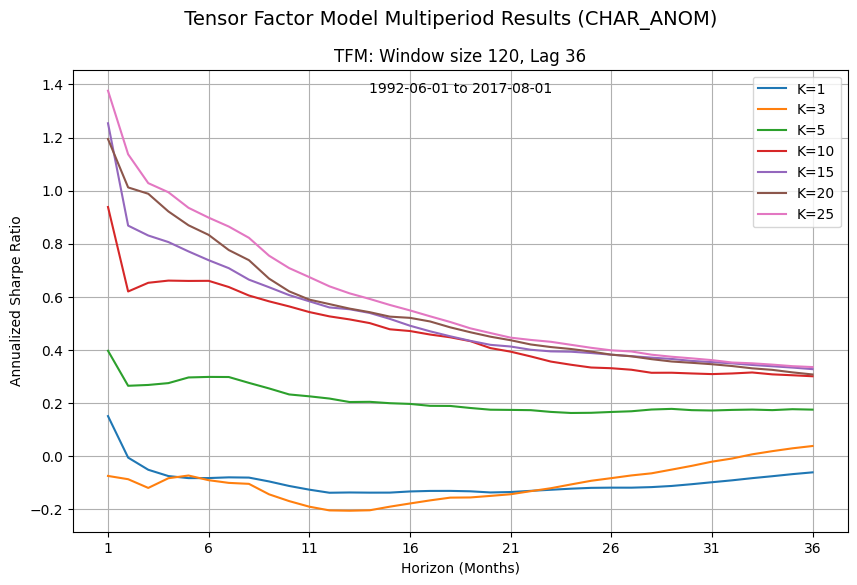
\includegraphics[width=1\linewidth]{full/char_anom_tensor_TFM.png}
    \caption{(CA) Tensor Factor Model: Full-Sample Sharpe Ratio}
    \label{fig:char_anom-primary-tfm}
\end{figure}

\begin{figure}[H]
    \centering
    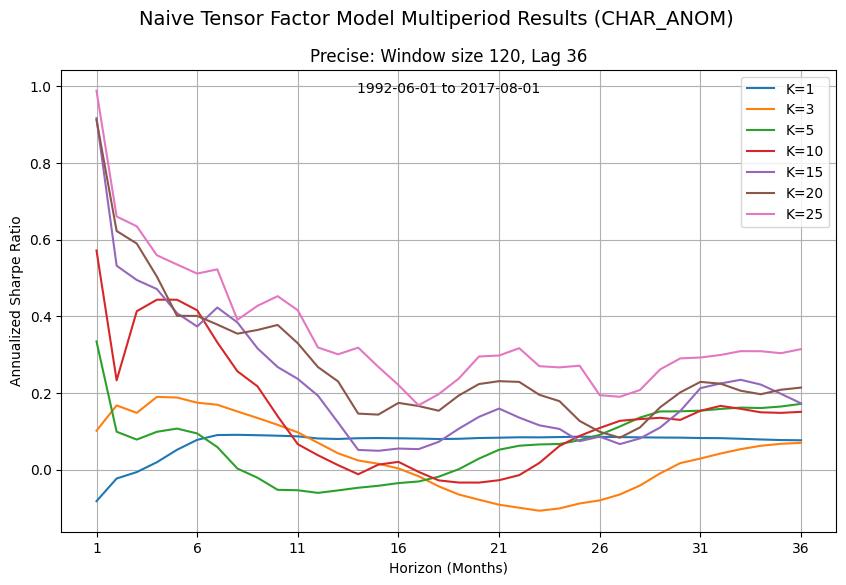
\includegraphics[width=1\linewidth]{full/char_anom_tensor_Precise.png}
    \caption{(CA) Precise Tensor Factor Model: Full-Sample Sharpe Ratio}
    \label{fig:char_anom-primary-precise}
\end{figure}

% \begin{figure}[H]
%     \centering
%     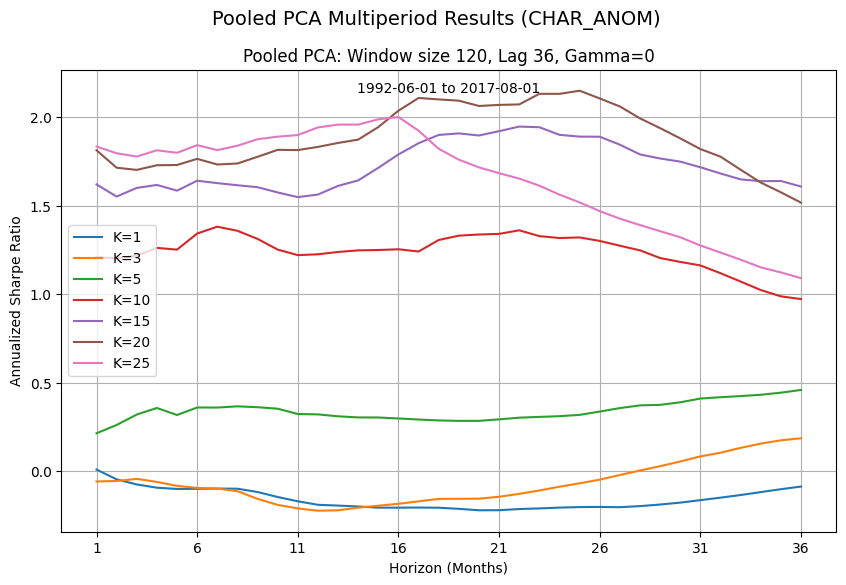
\includegraphics[width=1\linewidth]{full/char_anom_pooled_pca.png}
%     \caption{(CA) Pooled PCA Model: Full-Sample Sharpe Ratio}
%     \label{fig:char_anom-primary-pooled-pca}
% \end{figure}

\begin{figure}[H]
    \centering
    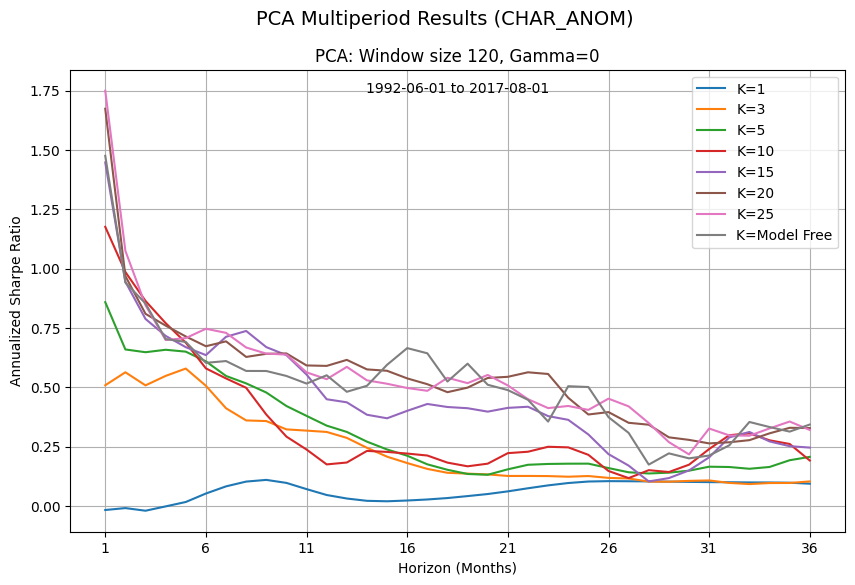
\includegraphics[width=1\linewidth]{full/char_anom_pca.png}
    \caption{(CA) Multiperiod PCA Model: Full-Sample Sharpe Ratio}
    \label{fig:char_anom-primary-pca}
\end{figure}


maybe a table that's like 

model $\implies$ K value (or model-free) $\implies$ sharpes for all 36 horizons

\subsubsection{Full-Sample SCS Dataset}

\begin{figure}[H]
    \centering
    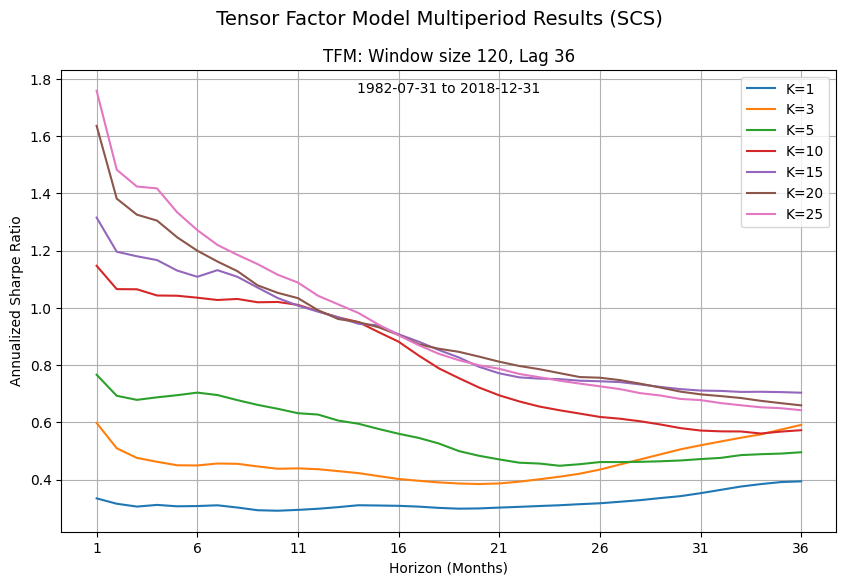
\includegraphics[width=1\linewidth]{full/scs_tensor_TFM.png}
    \caption{(SCS) Tensor Factor Model: Full-Sample Sharpe Ratio}
    \label{fig:scs-primary-tfm}
\end{figure}

\begin{figure}[H]
    \centering
    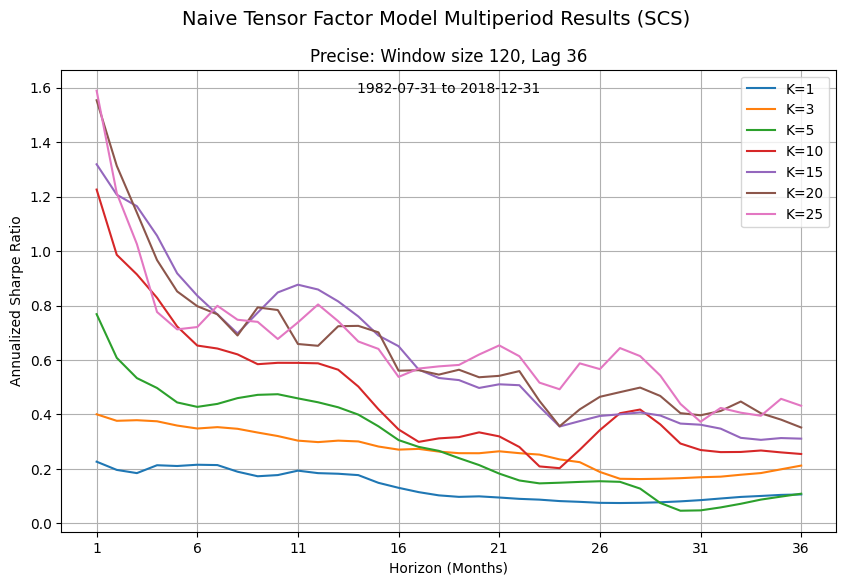
\includegraphics[width=1\linewidth]{full/scs_tensor_Precise.png}
    \caption{(SCS) Precise Tensor Factor Model: Full-Sample Sharpe Ratio}
    \label{fig:scs-primary-precise}
\end{figure}

% \begin{figure}[H]
%     \centering
%     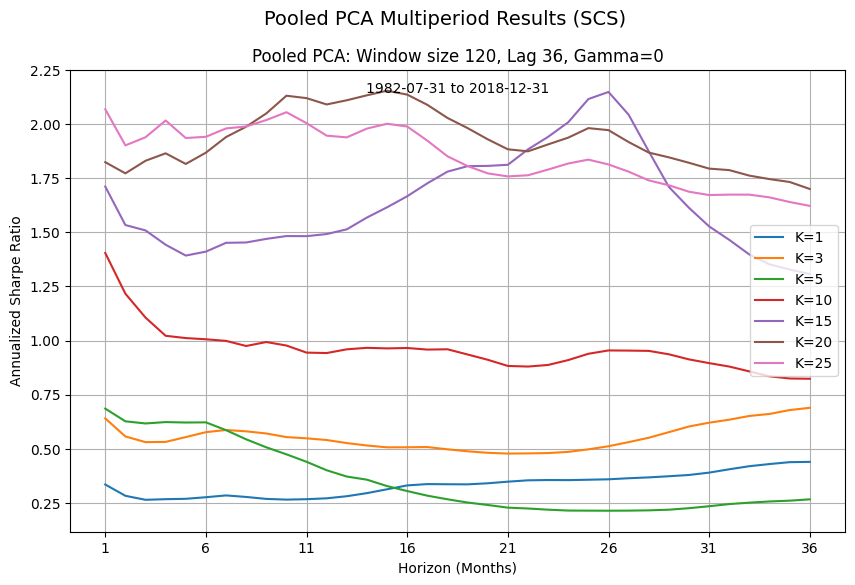
\includegraphics[width=1\linewidth]{full/scs_pooled_pca.png}
%     \caption{(SCS) Pooled PCA Model: Full-Sample Sharpe Ratio}
%     \label{fig:scs-primary-pooled-pca}
% \end{figure}

\begin{figure}[H]
    \centering
    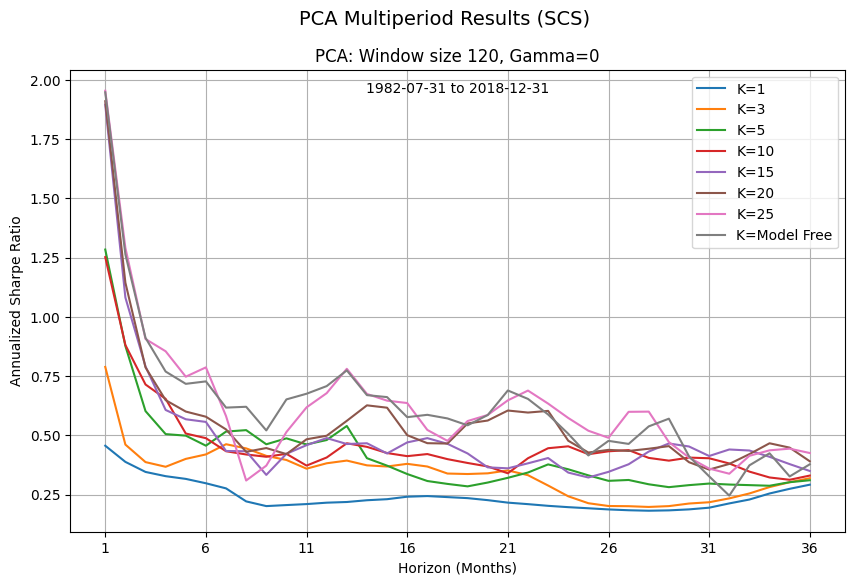
\includegraphics[width=1\linewidth]{full/scs_pca.png}
    \caption{(SCS) Multiperiod PCA Model: Full-Sample Sharpe Ratio}
    \label{fig:scs-primary-pca}
\end{figure}


\subsubsection{Full-Sample WRDS Dataset}

\begin{figure}[H]
    \centering
    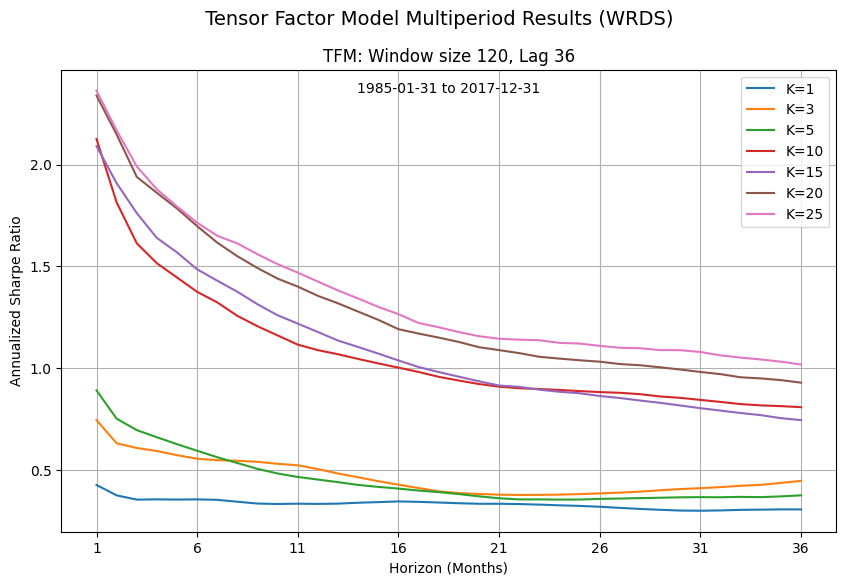
\includegraphics[width=1\linewidth]{full/wrds_tensor_TFM.png}
    \caption{(WRDS) Tensor Factor Model: Full-Sample Sharpe Ratio}
    \label{fig:wrds-primary-tfm}
\end{figure}

\begin{figure}[H]
    \centering
    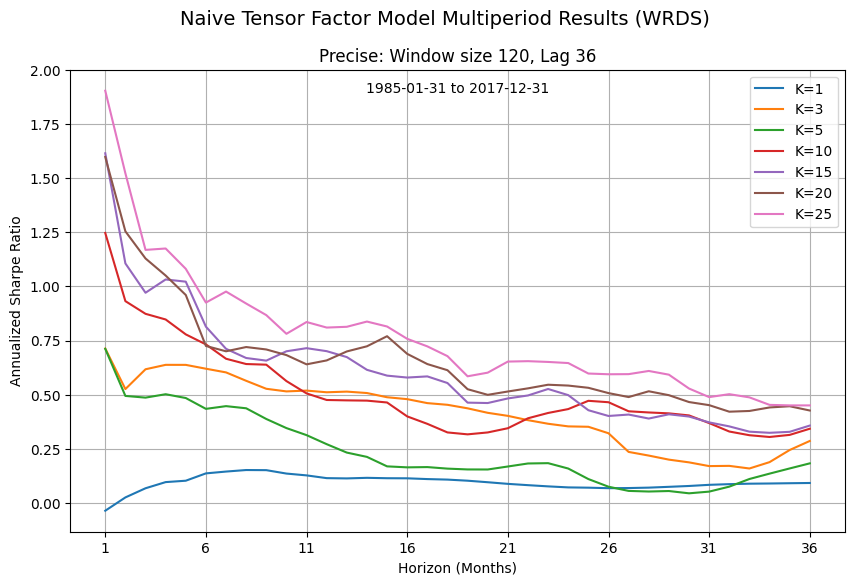
\includegraphics[width=1\linewidth]{full/wrds_tensor_Precise.png}
    \caption{(WRDS) Precise Tensor Factor Model: Full-Sample Sharpe Ratio}
    \label{fig:wrds-primary-precise}
\end{figure}

% \begin{figure}[H]
%     \centering
%     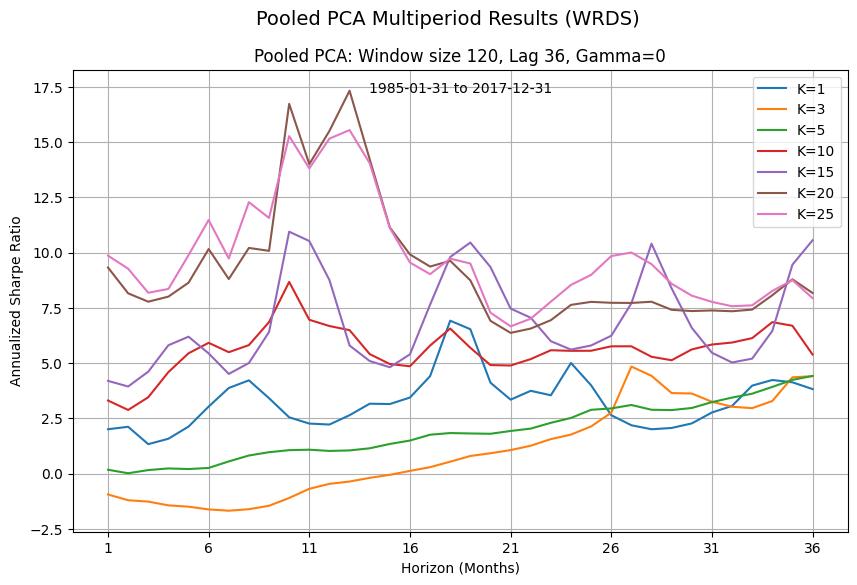
\includegraphics[width=1\linewidth]{full/wrds_pooled_pca.png}
%     \caption{(WRDS) Pooled PCA Model: Full-Sample Sharpe Ratio}
%     \label{fig:wrds-primary-pooled-pca}
% \end{figure}

\begin{figure}[H]
    \centering
    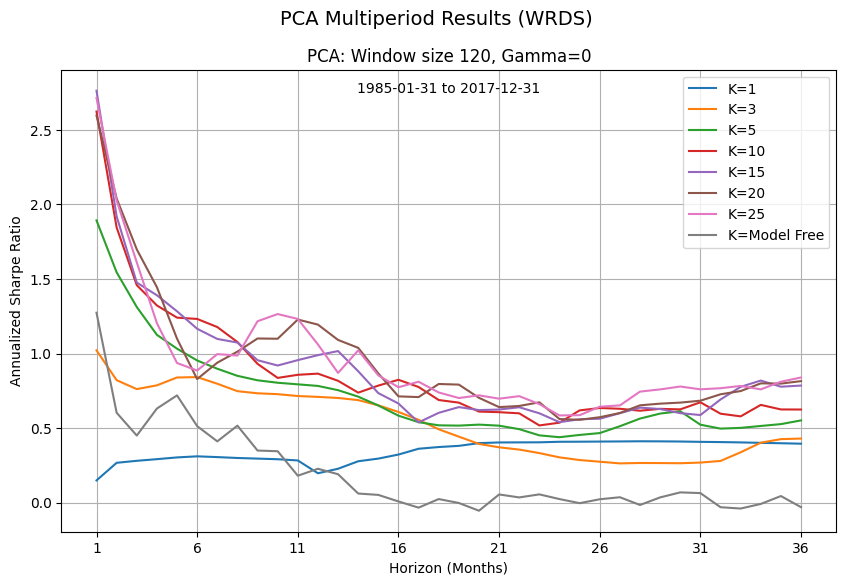
\includegraphics[width=1\linewidth]{full/wrds_pca.png}
    \caption{(WRDS) Multiperiod PCA Model: Full-Sample Sharpe Ratio}
    \label{fig:wrds-primary-pca}
\end{figure}


\subsubsection{Full-Sample Fama French 5 with Momentum Dataset}

\begin{figure}[H]
    \centering
    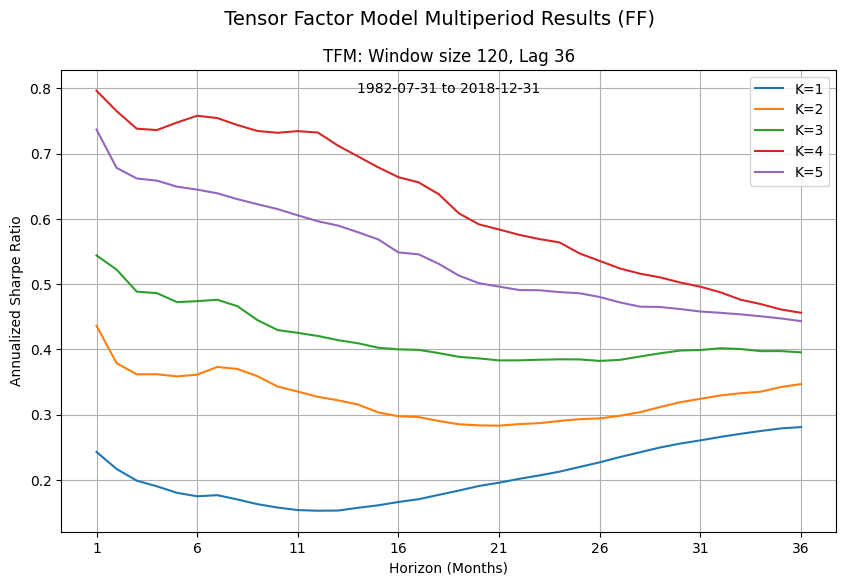
\includegraphics[width=1\linewidth]{full/ff_tensor_TFM.png}
    \caption{(FF5) Tensor Factor Model: Full-Sample Annualized SR}
    \label{fig:ff-primary-tfm}
\end{figure}

\begin{figure}[H]
    \centering
    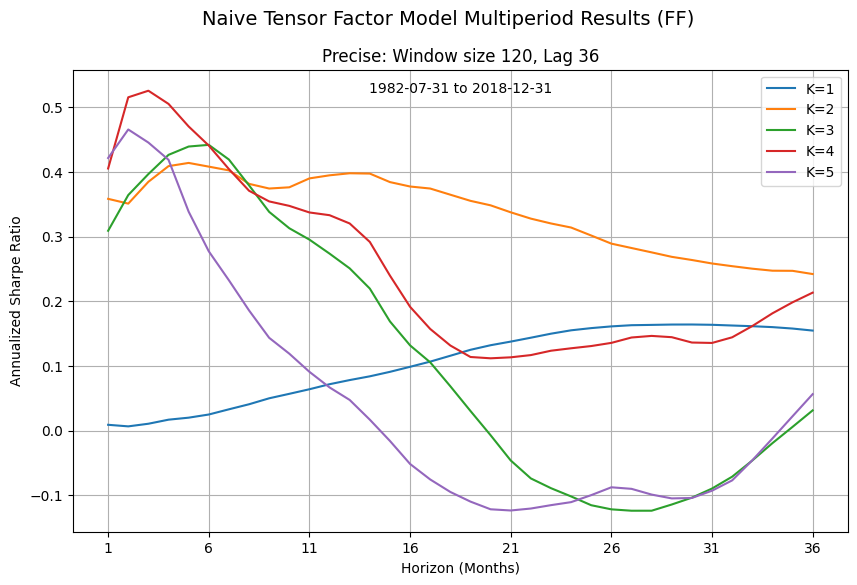
\includegraphics[width=1\linewidth]{full/ff_tensor_Precise.png}
    \caption{(FF5) Precise Tensor Factor Model: Full-Sample Annualized SR}
    \label{fig:ff-primary-precise}
\end{figure}

% \begin{figure}[H]
%     \centering
%     \includegraphics[width=1\linewidth]{full/ff_pooled_pca.png}
%     \caption{(FF5) Pooled PCA Model: Full-Sample Annualized SR}
%     \label{fig:ff-primary-pooled-pca}
% \end{figure}

\begin{figure}[H]
    \centering
    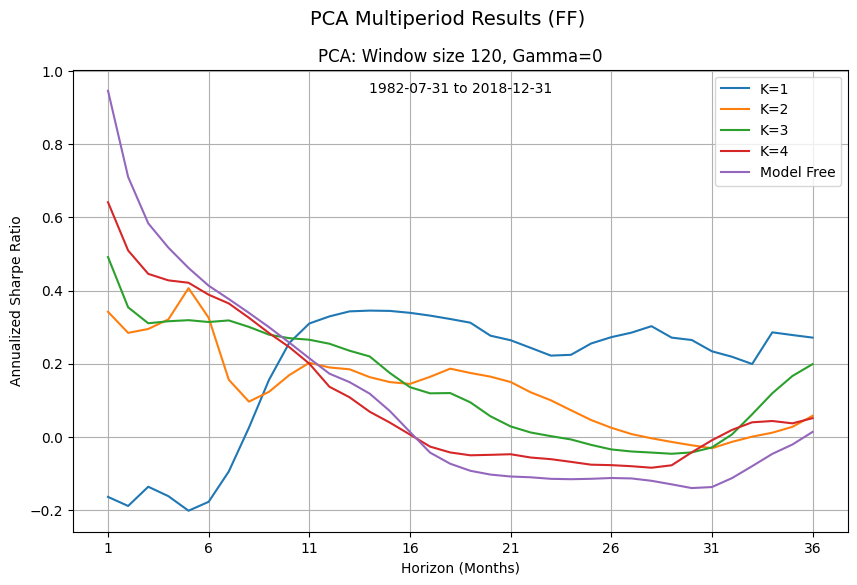
\includegraphics[width=1\linewidth]{full/ff_pca.png}
    \caption{(FF5) Multiperiod PCA Model: Full-Sample Annualized SR}
    \label{fig:ff-primary-pca}
\end{figure}


\newpage

\section{Appendix A}

\subsection{Primary Specification: OOS Results}

\subsubsection{OOS Characteristic Anomalies Dataset}

\begin{figure}[H]
    \centering
    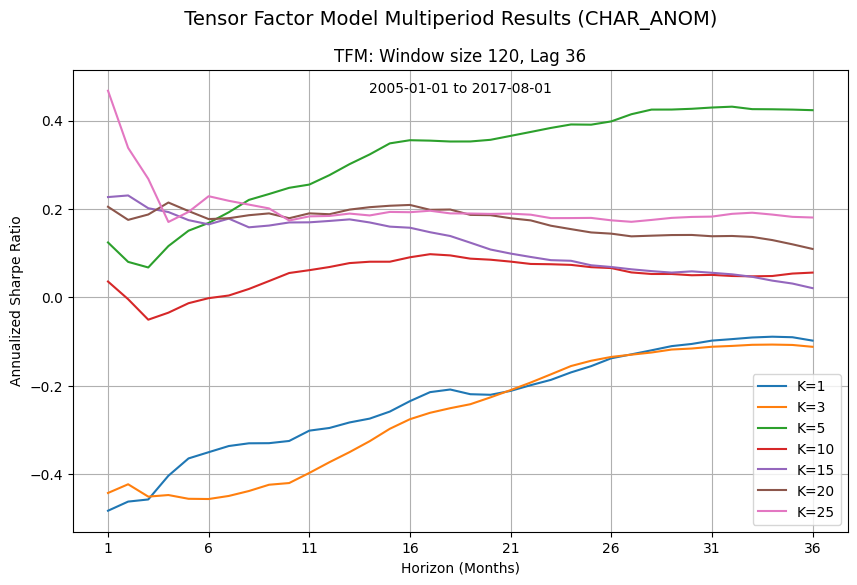
\includegraphics[width=1\linewidth]{oos/char_anom_tensor_TFM.png}
    \caption{(CA) Tensor Factor Model: OOS Annualized SR}
    \label{fig:char_anom-oos-tfm}
\end{figure}

\begin{figure}[H]
    \centering
    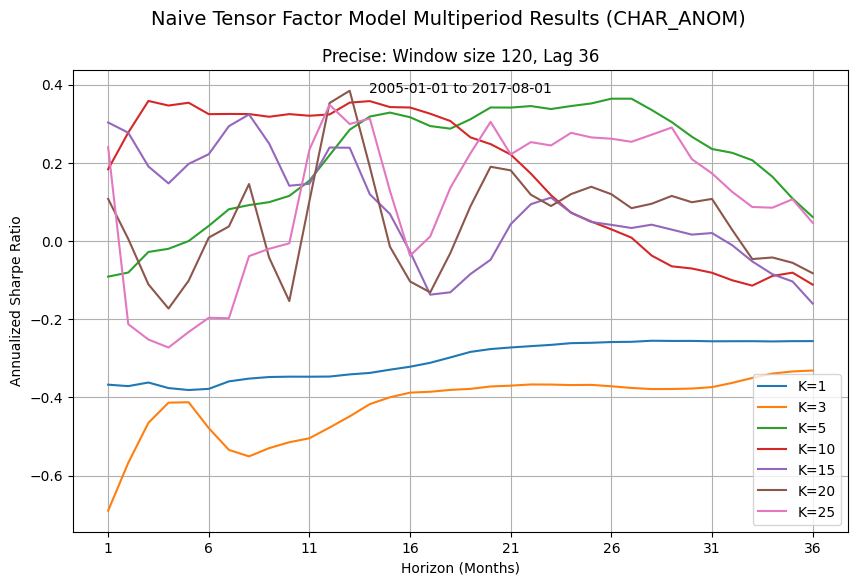
\includegraphics[width=1\linewidth]{oos/char_anom_tensor_Precise.png}
    \caption{(CA) Precise Tensor Factor Model: OOS Annualized SR}
    \label{fig:char_anom-oos-precise}
\end{figure}

% \begin{figure}[H]
%     \centering
%     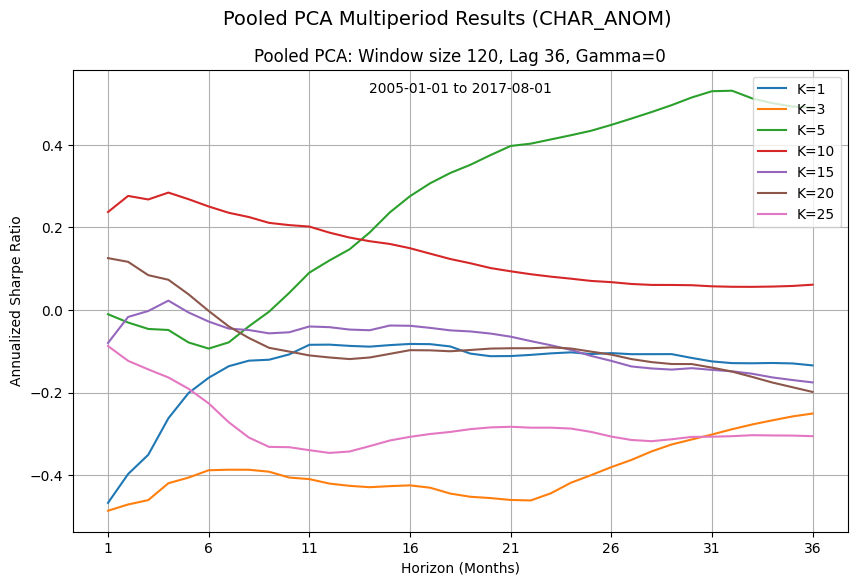
\includegraphics[width=1\linewidth]{oos/char_anom_pooled_pca.png}
%     \caption{(CA) Pooled PCA Model: OOS Annualized SR}
%     \label{fig:char_anom-oos-pooled-pca}
% \end{figure}

\begin{figure}[H]
    \centering
    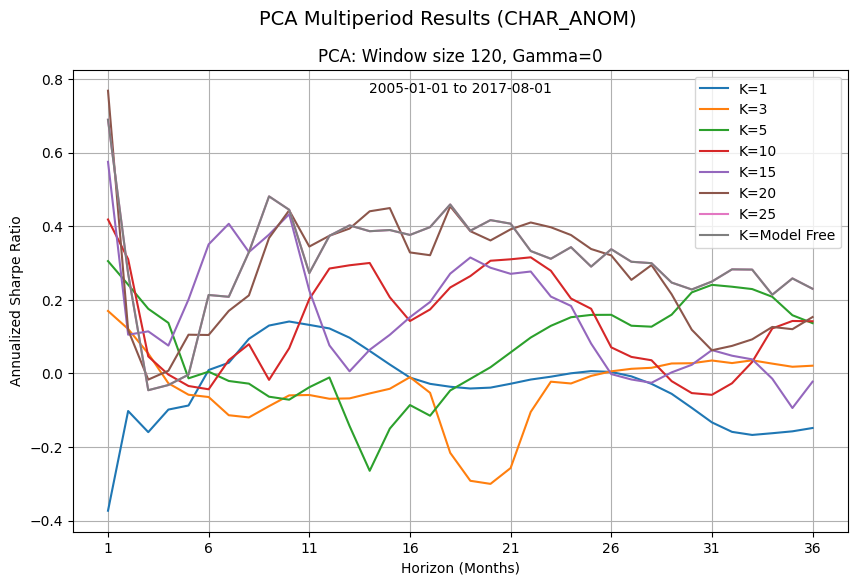
\includegraphics[width=1\linewidth]{oos/char_anom_pca.png}
    \caption{(CA) Multiperiod PCA Model: OOS Annualized SR}
    \label{fig:char_anom-oos-pca}
\end{figure}
    

\subsubsection{OOS SCS Dataset}

\begin{figure}[H]
    \centering
    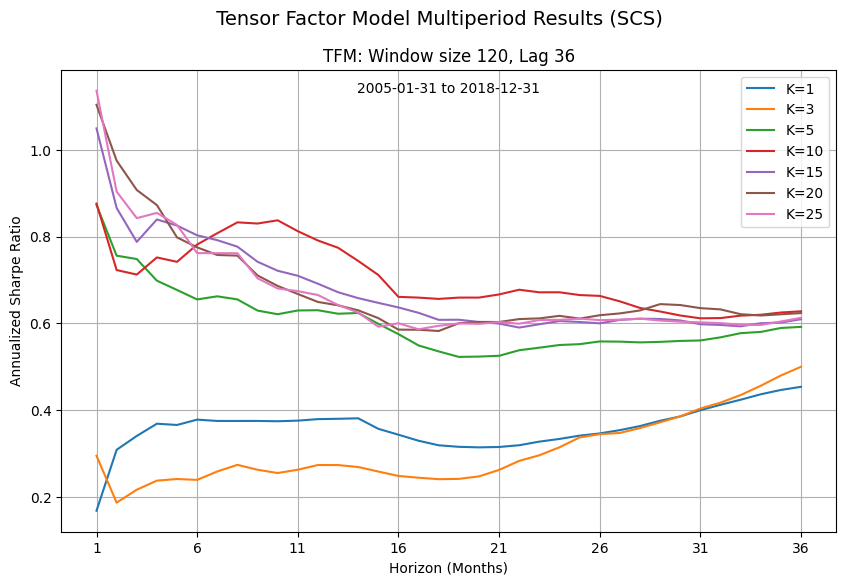
\includegraphics[width=1\linewidth]{oos/scs_tensor_TFM.png}
    \caption{(SCS) Tensor Factor Model: OOS Annualized SR}
    \label{fig:scs-oos-tfm}
\end{figure}

\begin{figure}[H]
    \centering
    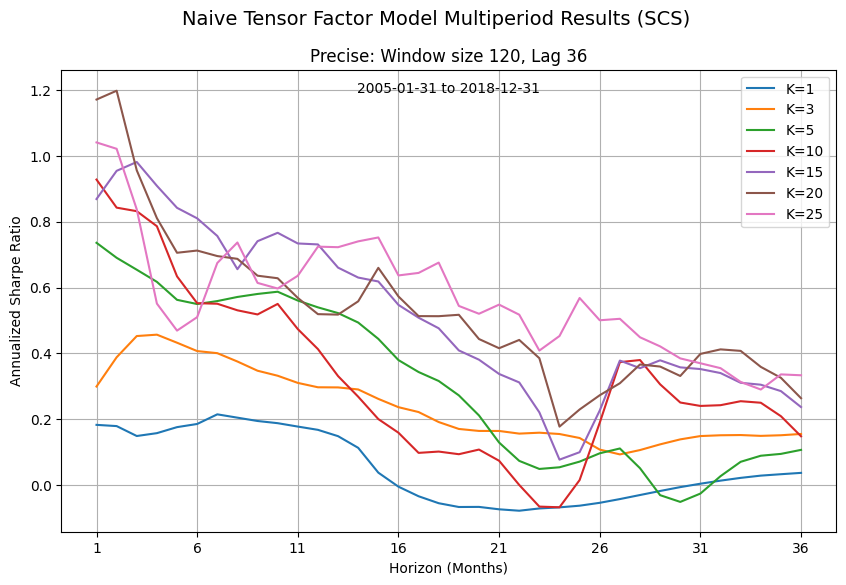
\includegraphics[width=1\linewidth]{oos/scs_tensor_Precise.png}
    \caption{(SCS) Precise Tensor Factor Model: OOS Annualized SR}
    \label{fig:scs-oos-precise}
\end{figure}

% \begin{figure}[H]
%     \centering
%     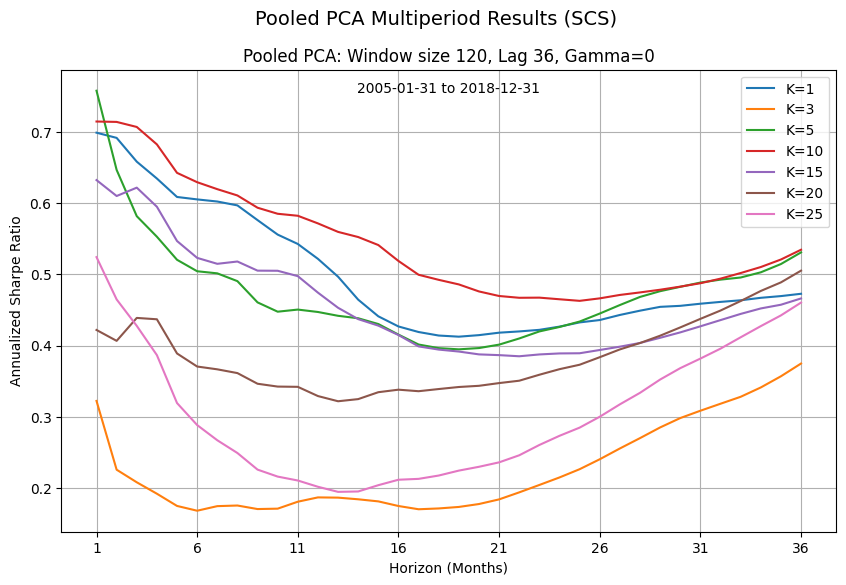
\includegraphics[width=1\linewidth]{oos/scs_pooled_pca.png}
%     \caption{(SCS) Pooled PCA Model: OOS Annualized SR}
%     \label{fig:scs-oos-pooled-pca}
% \end{figure}

\begin{figure}[H]
    \centering
    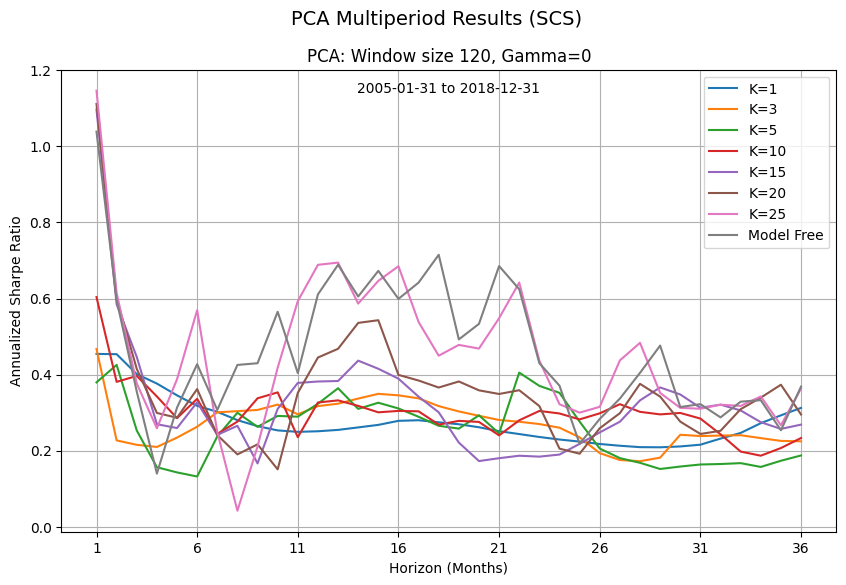
\includegraphics[width=1\linewidth]{oos/scs_pca.png}
    \caption{(SCS) Multiperiod PCA Model: OOS Annualized SR}
    \label{fig:scs-oos-pca}
\end{figure}


\subsubsection{OOS WRDS Dataset}

\begin{figure}[H]
    \centering
    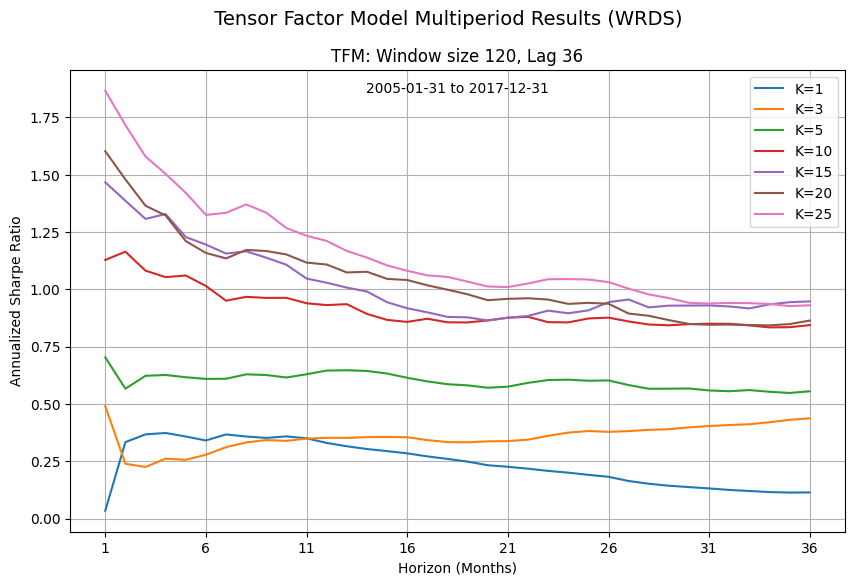
\includegraphics[width=1\linewidth]{oos/wrds_tensor_TFM.png}
    \caption{(WRDS) Tensor Factor Model: OOS Annualized SR}
    \label{fig:wrds-oos-tfm}
\end{figure}

\begin{figure}[H]
    \centering
    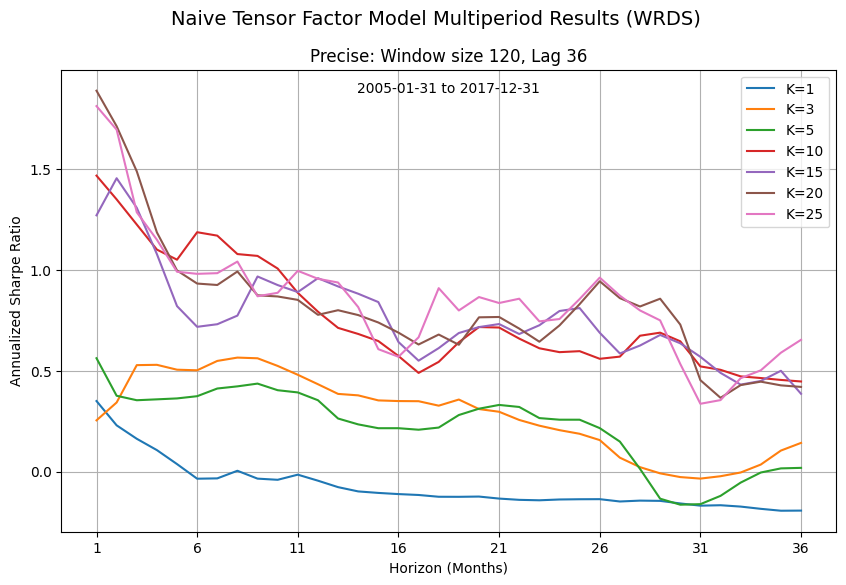
\includegraphics[width=1\linewidth]{oos/wrds_tensor_Precise.png}
    \caption{(WRDS) Precise Tensor Factor Model: OOS Annualized SR}
    \label{fig:wrds-oos-precise}
\end{figure}

% \begin{figure}[H]
%     \centering
%     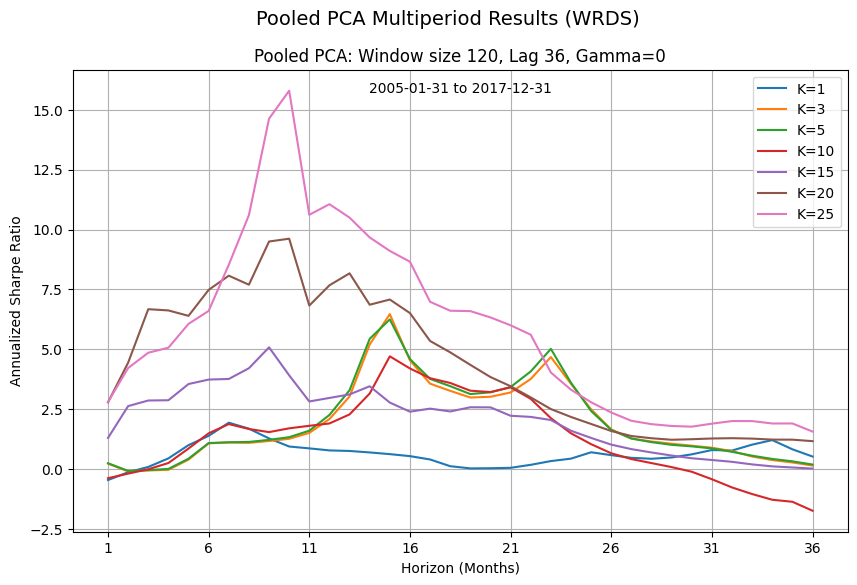
\includegraphics[width=1\linewidth]{oos/wrds_pooled_pca.png}
%     \caption{(WRDS) Pooled PCA Model: OOS Annualized SR}
%     \label{fig:wrds-oos-pooled-pca}
% \end{figure}

\begin{figure}[H]
    \centering
    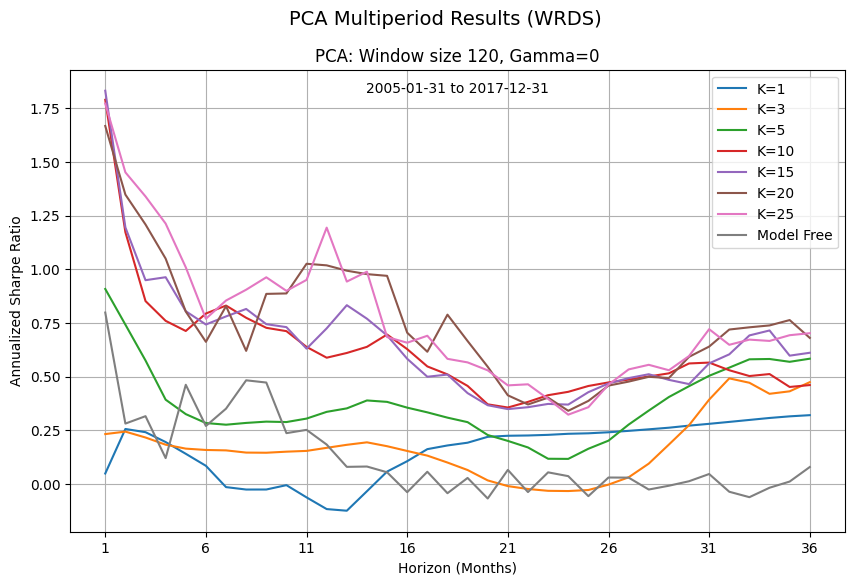
\includegraphics[width=1\linewidth]{oos/wrds_pca.png}
    \caption{(WRDS) Multiperiod PCA Model: OOS Annualized SR}
    \label{fig:wrds-oos-pca}
\end{figure}


\subsubsection{Post-2005 Fama French 5 with Momentum Dataset}

\begin{figure}[H]
    \centering
    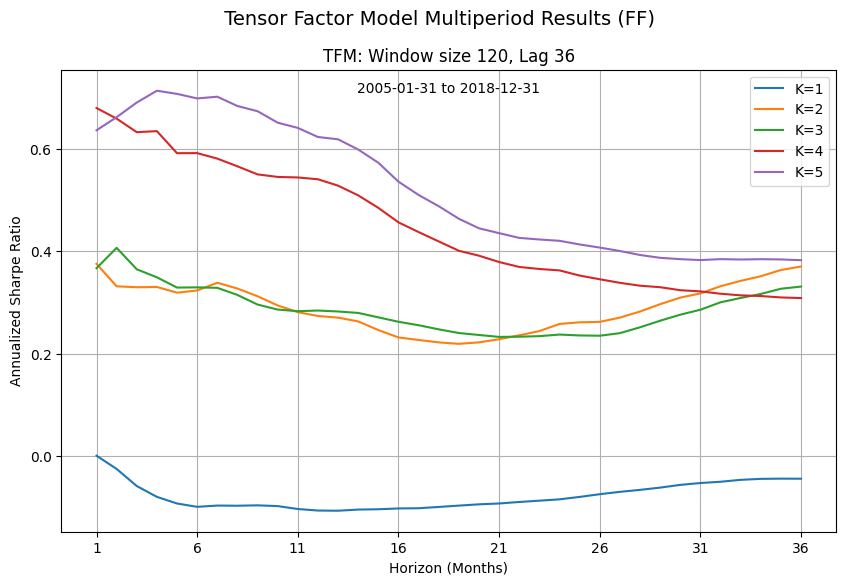
\includegraphics[width=1\linewidth]{post-2005/ff_tensor_TFM.png}
    \caption{(FF5) Tensor Factor Model: Post-2005 Sharpe Ratio}\label{fig:ff-post-2005-tfm}
\end{figure}

\begin{figure}[H]
    \centering
    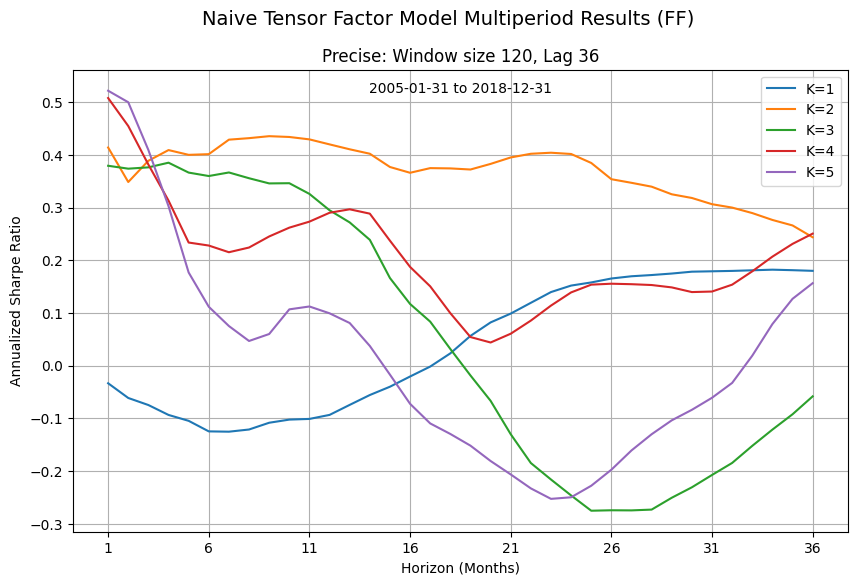
\includegraphics[width=1\linewidth]{post-2005/ff_tensor_Precise.png}
    \caption{(FF5) Precise Tensor Factor Model: Post-2005 Sharpe Ratio}\label{fig:ff-post-2005-precise}
\end{figure}

% \begin{figure}[H]
%     \centering
%     \includegraphics[width=1\linewidth]{post-2005/ff_pooled_pca.png}
%     \caption{(FF) Pooled PCA Model: Post-2005 Sharpe Ratio}
%     \label{fig:ff-post-2005-pooled-pca}
% \end{figure}

\begin{figure}[H]
    \centering
    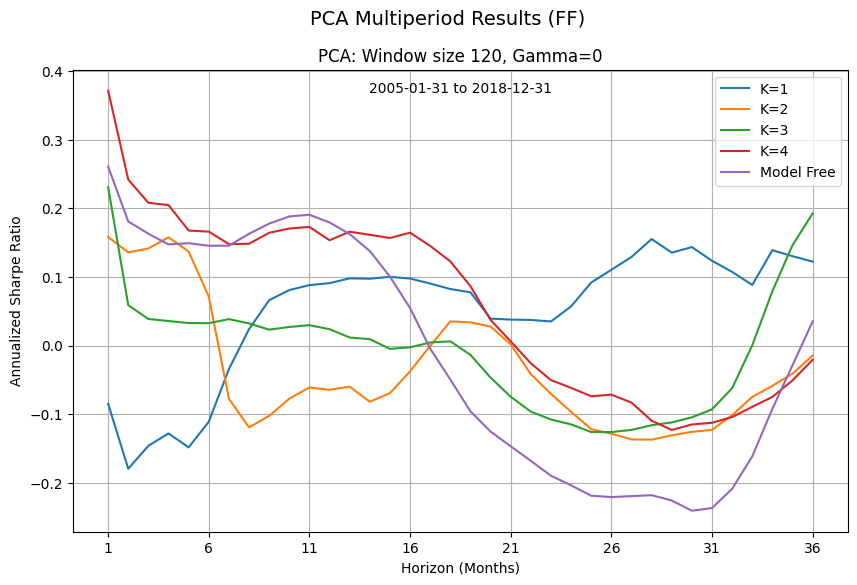
\includegraphics[width=1\linewidth]{post-2005/ff_pca.png}
    \caption{(FF5) Multiperiod PCA Model: Post-2005 Sharpe Ratio}\label{fig:ff-post-2005-pca}
\end{figure}


\newpage
% \section{Appendix B}

% \[\Lambda w_n = w_k \implies w_n = \Lambda_k^\dagger w_k\]
% \[w_n = \Lambda_k(\Lambda_k^T \Lambda_k)^{-1} w_k\]

\section{Appendix B}

% \begin{lemma} \label{misc-lemma}
%     For any two real symmetric square matrices $A, B \in \R^{N \times N}$ and $y \in \R^N$
%     \[(A \cdot B) y = diag(A D_y B^T)\]
% \begin{proof}
%     Note that the element of $(A \cdot B)_{i, j} = A_{i, j} \cdot B_{i, j}$
%     Furthermore, the product with vector $y$ results in a vector $v$ where 
%     \[v_i = \sum_j (A_{i, j} \cdot B_{i, j}) \cdot y_j\]
%     Now observe the other side. $D_y$ is a diagonal matrix, so $AD_y$ scales each column $j$ 
%     of $A$ by $y_j$; thus, $(AD_y)_{i, j} = A_{i, j} \cdot y_j$. $B^\top$ is the transpose of $B$
%     so $(B^\top)_{j, i} = B_{i, j}$. This product $AD_y B^\top$ results in a matrix $M$
%     where each $M_{i, i}$ is 
%     \[M_{i, i} = \sum_j (A_{i, j} \cdot y_j) \cdot B_{i, j}\]
%     Thus, $v = diag(M)$ and so we are done. 
% \end{proof}
% \end{lemma}

\begin{lemma} \label{elementwise-ruins-everything}
    There does not exist a closed-form solution of $(A \cdot B)^{-1}$ where 
    $A, B \in \R^{N \times N}$ and are real and symmetric and $\cdot$ is element-wise multiplication. 
    \begin{proof}
        Consider a counter-example where
        \begin{align*}
            A = \begin{pmatrix}
                1 & 0\\
                0 & 1
            \end{pmatrix} && B = \begin{pmatrix}
                0 & 1\\
                1 & 0
            \end{pmatrix}
        \end{align*}
        Clearly, $A$ and $B$ are both invertible, but $(A \cdot B)$ is not invertible, 
        and thus we cannot even guarantee existence, much less uniqueness.
    \end{proof}
\end{lemma}
    
\begin{lemma} \label{outer-prod-elementwise-trick}
    For two vectors $x, y \in \R^N$ and a square matrix $A \in \R^{N \times N}$, then 
    \[(yx^\top) \cdot A = D_y A D_x^\top\]
    where $D_y \in \R^{N \times N}$ matrix the elements of $y$ along the diagonal and $0$ elsewhere. 

    \begin{proof}
        Omitted. Found on Wikipedia page for Hadamard products.
    \end{proof}
\end{lemma}

% \begin{lemma}[Miller's Lemma]
%     If $G$ is rank $n$ and $H$ is rank one, then 
%     \[(G + H)^{-1} = G^{-1} - \frac{1}{1 + g}G^{-1} H G^{-1}\]
%     where $g = \text{tr}(HG^{-1})$

%     \begin{proof}
%         See Miller.

%         In our case, $G$ would have the form $G = D_{W_l} \Sigma D_{W_l}$ and so substituting this into the above yields 
%         \begin{align}
%             (G + H)^{-1} = D_{W_l}^{-1} \Sigma^{-1} D_{W_l}^{-1} - \frac{1}{1 + g} D_{W_l}^{-1} \Sigma^{-1} D_{W_l}^{-1} H D_{W_l}^{-1} \Sigma^{-1} D_{W_l}^{-1}
%         \end{align}
%     \end{proof}
% \end{lemma}

% \begin{theorem}[Miller's Theorem]
%     Let $G$ and $G + H$ be nonsingular matrices and let $H$ have positive rank $r$. Let $H = E_1 + E_2 + \cdots + E_r $, 
%     where each $E_k $ has rank one and $C_{k+1} = G + E_1 + \cdots + E_k$ is nonsingular for $k = 1, \ldots, r$. Then if $C_1 = G$,
% \[ C_{k+1}^{-1} = C_k^{-1} - \nu_k C_k^{-1} E_k C_k^{-1}, \quad k = 1, \ldots, r \]
% where
% \[ \nu_k = \frac{1}{1 + \text{tr} \, C_k^{-1} E_k}. \]
% In particular,
% \[ (G + H)^{-1} = C_r^{-1} - \nu_r C_r^{-1} E_r C_r^{-1}. \]

% \begin{proof}
%     To prove this result we first write $C_2 = C_1 + E_1 = G + E_1$ and recall that $G$ and $C_2$ are nonsingular. Then by the Lemma,
%     \[C_2^{-1} = G^{-1} - \nu_1 G^{-1} E_1 G^{-1}\]
%     and we have calculated $C_2^{-1} $in terms of $G^{-1}$. Now $C_3 = G + E_1 + E_2 = C_2 + E_2$. Hence since $C_2 $and $C_3$ are nonsingular, we again may invoke the Lemma to write $C_3^{-1} $in terms of $C_2^{-1} $
%     \[ C_3^{-1} = C_2^{-1} - \nu_2 C_2^{-1} E_2 C_2^{-1}. \]
%     But $C_2^{-1}$, and if we continue this process $r $times (where $r $is the rank of $H$) we obtain
%     \[ C_{r+1}^{-1} = C_r^{-1} - \nu_r C_r^{-1} E_r C_r^{-1}. \]
%     But $C_{r+1} = G + H$, and thus our Theorem is proved.
% \end{proof}
% \end{theorem}

% \begin{theorem}[Henderson and Searle Theorem]
%     If $A$ and $B$ are symmetric, (as they are in our case), then 
    

%     \begin{proof}
%         Omitted. In 
%     \end{proof}
% \end{theorem}


\begin{note}[Multihorizon Covariance Matrix]
We want to analyze equation \ref{cov}.

\begin{proof}[Solution]
By Lemma \ref{outer-prod-elementwise-trick}, each term in the summation simplifes such that
\[\left( \left( \sum_{l=1}^S (W_l W_l^\top)\right) \cdot \text{Var}(F_t)\right)^{-1}  = \left( \sum_{l=1}^S D_{W_l} \text{Var}(F_t) D_{W_l}\right)^{-1}\]
Now consider the eigendecomposition of the covariance matrix (which is positive semi-definite) $\text{Var}(F_t) = Q\Lambda Q^\top$
where the columns of $Q$ are the eigenvectors. 
\[\left( \sum_{l=1}^S D_{W_l} Q \Lambda Q^\top D_{W_l}\right)^{-1}\]
If all of the eigenvalues in $\Lambda$ are distinct (which should be reasonable despite the 
lack of orthogonality between the factors in PARAFAC), then $Q$ is orthogonal and by definition, 
$Q^\top = Q^{-1}$. Thus, $Q^\top D_{W_l} = Q^{-1} D_{W_l}$ maps each of the columns of $D_{W_l}$
onto the eigenspace spanned by the eigenvectors of the covariance matrix. 

The mapping of $D_{W_l}$ onto the eigenspace spanned by the covariance matrix’s eigenvectors suggests a powerful economic interpretation. 
This transformation effectively decomposes the investment horizon weights into the same coordinate system where risk factors naturally vary. 
This means we’re aligning our investment horizons with the fundamental modes of variation in the underlying factors.

Let $X_l = Q^T D_{W_l}$, which is now neither diagonal orthogonal, or symmetric. Now we have 
\[\left( \sum_{l=1}^S X_l^\top \Lambda X_l \right)^{-1}\]

Note that for some $l$, $X_l^\top \Lambda X_l$ is a positive semi-definite matrix because the eigenvalues 
in $\Lambda$ are guaranteed to be nonnegative, and furthermore, the sum of PSD matrices is still PSD. The fact that the sum of PSD matrices remains PSD ensures that the portfolio's risk remains 
well-defined and manageable. This is crucial in mean-variance optimization, as it guarantees that the covariance matrix used in the optimization process is valid.
\end{proof}
\end{note}



\begin{note}[PSD Stability]


\begin{proof}[Solution]

Recall that the covariance matrix is PSD, so eigenvalues are all nonnegative, and $\Lambda$ is diagonal and therefore symmetric.
The sum of PSD matrices is still PSD. Alternatively, just from \ref{cov} each element in the outer product is positive 
so when multiplied by the covariance matrix, one would propose that the result was PSD but this shows it. 

\hfill

We have the following equality

Further exploring, this could be a deadend, is there some nice assumption
\begin{align*}
    \left( \sum_{l=1}^S X_l^\top \Lambda X_l \right)^{(i, j)} &= \sum_{k=1}^K \Lambda_k \left(\sum_{l=1}^S X_l^{(k, i)} X_l^{(k, j)}\right)\\
    &= \sum_{k=1}^K \Lambda_k 
\end{align*}
Each $X_l^{(i, j)} = \sum_{k=1}^K Q^{(k, i)} D_{W_l}^{(k, j)} $
\end{proof}
\end{note}



\end{document}
